\documentclass{beamer}
\usepackage[spanish]{babel}
\usepackage{beamerthemeshadow}
\usepackage{pgf}
\usepackage{eurosym}
\usepackage{array}% http://ctan.org/pkg/array
\usepackage{fontspec}
\usepackage{fontawesome}
\newcolumntype{M}{>{\centering\arraybackslash}m{\dimexpr.25\linewidth-2\tabcolsep}}
\usepackage{hyperref}
\hypersetup{
  breaklinks=true,
  urlcolor=blue,
}

\usetheme{CambridgeUS}
\usefonttheme{structurebold}

\setbeamertemplate{itemize item}[triangle]

\begin{document}


\title{Sistemas de control de versiones distribuidos}
\subtitle{Controla las versiones de tu trabajo con GIT}
\author[Nacho Álvarez]{\texorpdfstring{Nacho Álvarez
  \\ \faTwitter \hspace{5pt}@neonigmacdb
  \\ \faEnvelope \hspace{5pt}neonigma@gmail.com}{Author}}

\institute[WUL4]{
\includegraphics[height=0.6cm]{imgs/wul4.png}}
\date{\today}



\frame{\centering 
\includegraphics[height=1cm]{imgs/training-thursday.png} \titlepage}

\section[Índice]{}
\frame{\tableofcontents}


\section{Acerca de mí}
\frame
{
\frametitle{Who?}
\begin{itemize}
\item \textbf{Trayectoria profesional:} soporte UCO, desarrollador Web, desarrollador / integrador distribuciones GNU/Linux.
\item \textbf{Actualmente:} WUL4 Córdoba (mobile + backend developer)
\item \textbf{Involucrado en:}
\begin{center}
  $\vcenter{\hbox{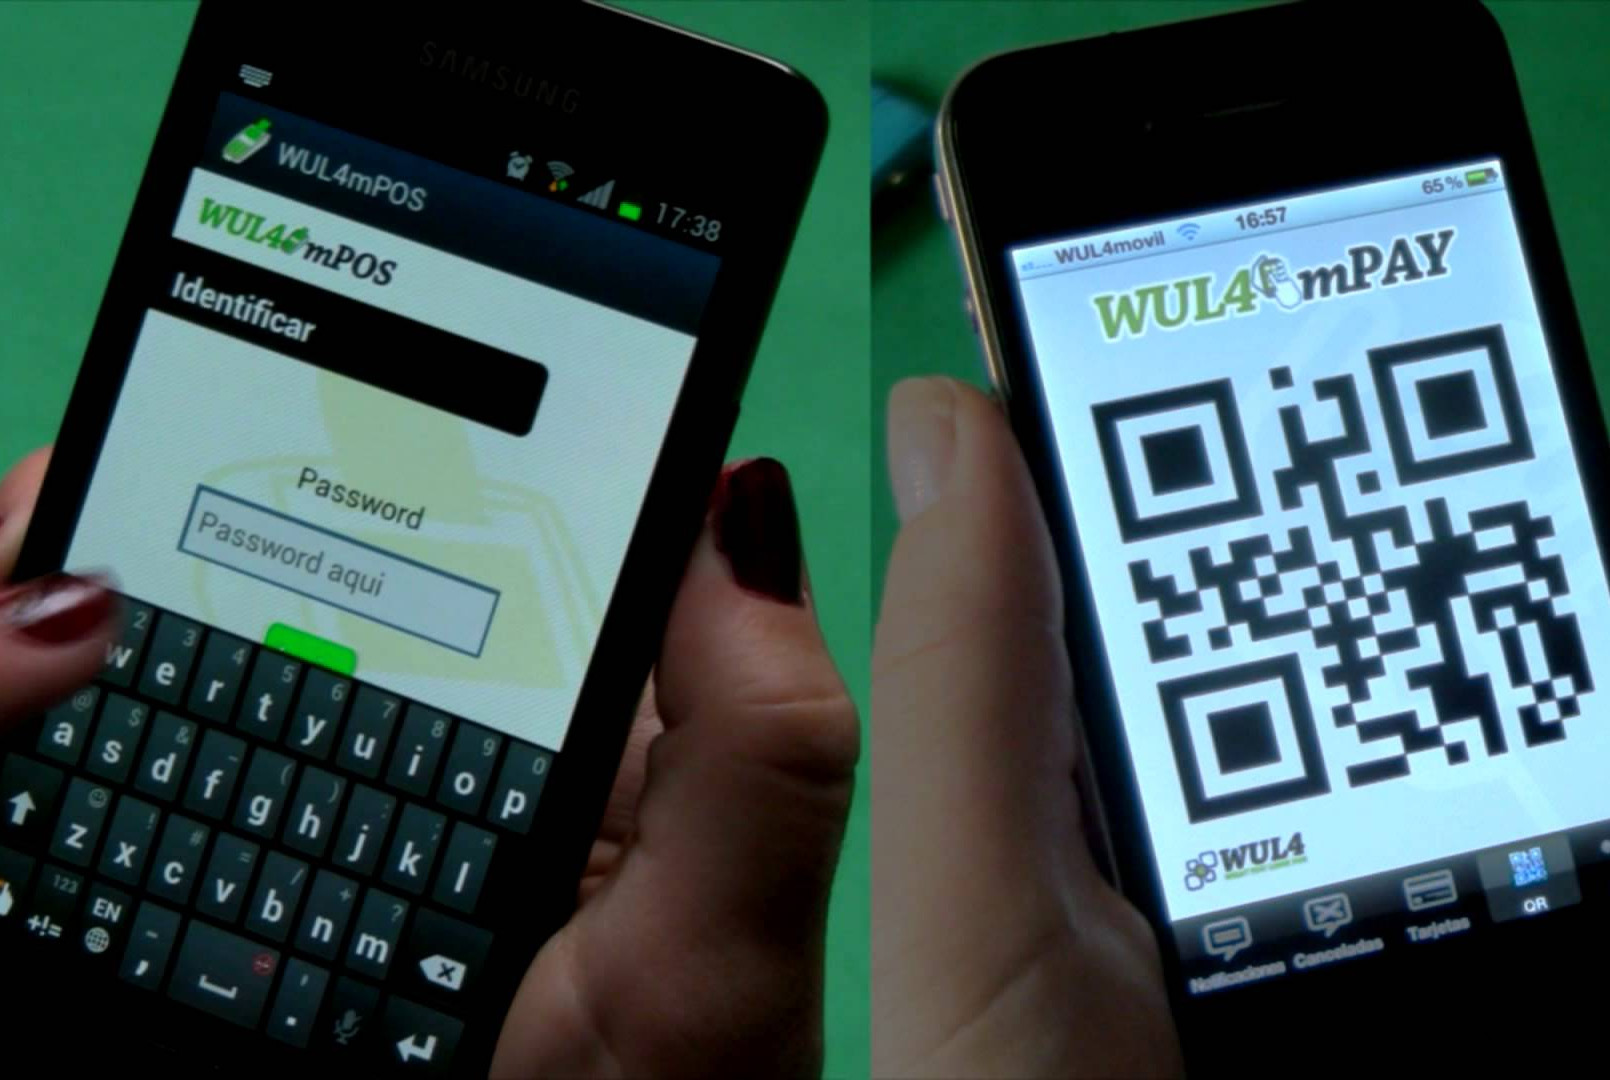
\includegraphics[height=1.25in,width=1.5in]{imgs/wul4mpay.jpg}}}$
  $\vcenter{\hbox{
\includegraphics[height=1.25in]{imgs/wul4bus.jpg}}}$
  $\vcenter{\hbox{
\includegraphics[height=1.25in]{imgs/id.jpg}}}$
  $\vcenter{\hbox{
\includegraphics[width=0.9in]{imgs/redsys.jpg}}}$
\end{center}
\end{itemize}
}

\section{Definiciones}
\frame
{
\frametitle{Definiciones}
\begin{itemize}
\item \textbf{Control de versiones:} gestión de los diversos cambios que se realizan sobre los elementos de algún producto
\item Una \textbf{versión}, \textbf{revisión} o \textbf{edición} de un producto, es el \textbf{estado} en el que se encuentra dicho producto en un \textbf{momento} dado de su desarrollo o modificación
\item Los \textbf{sistemas} de control de versiones (SCV) vienen a automatizar parcialmente la gestión de este control de cambios
\item Existen SCV \textbf{centralizados} (repositorio único remoto) y SCV \textbf{distribuidos} (cada usuario su repositorio local + remoto)
\item Los más famosos y de más trayectoria son: SVN, GIT, Mercurial, Bazaar, ClearCase, Perforce...
\end{itemize}
}

\section*{SCV centralizados}
\frame
{
\frametitle{Ventajas SCV centralizados}
\begin{itemize}
\item En los sistemas distribuidos hay un \textbf{mayor bloqueo} del estado final del proyecto que en los sistemas centralizados.
\item En los sistemas centralizados las versiones vienen identificadas por un \textbf{número de versión}. En lugar de eso, en los sistemas distribuidos, cada versión tiene un identificador (hash) al que se le puede asociar una etiqueta (tag).
\item La \textbf{curva de aprendizaje} es sensiblemente menor que en los sistemas distribuidos
\item Requiere \textbf{menor intervención} del mantenedor
\end{itemize}
}

\section*{SCV distribuidos}
\frame
{
\frametitle{Ventajas SCV distribuidos}
\begin{itemize}
\item Necesita \textbf{menos operaciones en red} => mayor autonomía y una mayor rapidez.
\item Aunque se \textbf{caiga} el \textbf{repositorio remoto} la gente puede seguir trabajando
\item Alta probabilidad de \textbf{reconstrucción} en caso de falla debido a su arquitectura distribuida
\item Permite mantener \textbf{repositorios centrales más limpios}, el mantenedor decide
\item El \textbf{servidor remoto} requiere \textbf{menos recursos} que los que necesitaría un servidor centralizado ya que gran parte del trabajo lo realizan los \textbf{repositorios locales}.
\item Al ser los sistemas distribuidos \textbf{más recientes} que los sistemas centralizados, y al tener \textbf{más flexibilidad} por tener un repositorio local y otro/s remotos, estos sistemas han sido diseñados para hacer fácil el uso de \textbf{ramas locales y remotas} (creación, evolución y fusión) y poder aprovechar al máximo su potencial. 
\end{itemize}
}

\section{¿Por qué GIT?}
\usebackgroundtemplate{%
  
\includegraphics[width=\paperwidth,height=\paperheight]{imgs/git-no.jpg}} 
\frame
{
\frametitle{¿Por qué GIT?}
}

\usebackgroundtemplate{%
  
\includegraphics[width=\paperwidth,height=\paperheight]{imgs/git-si.jpg}} 
\frame
{
\frametitle{¿Por qué GIT?}
}
\usebackgroundtemplate{}
\frame
{
\frametitle{En números}

\includegraphics[height=1cm]{imgs/git-bitbucket.png}
\begin{itemize}
 \item Enfocado a \textbf{código privado} (Facebook, Cisco, Adobe, Opera...)
 \item Más de \textbf{1 millón} de usuarios registrados
 \item Integración del resto del ecosistema software: Bamboo (CI), Confluence (Doc), Jira (project tracking), SourceTree (GUI)...
 \item Se cobra por \textbf{número de integrantes de equipo}: 0-5 (gratis), 6-10 (\$10 month), 11-25 (\$25 month), 26-50 (\$50 month)...
\end{itemize}


\includegraphics[height=1cm]{imgs/git-github.png}
\begin{itemize}
 \item Enfocado a \textbf{código abierto} (bootstrap, nodejs, jquery...)
 \item Más de \textbf{4 millones} de usuarios registrados y \textbf{8 millones} de \textbf{repositorios} creados
 \item Se cobra por \textbf{repositorios privados}: 5 (\$7 month), 10 (\$12 month), 20 (\$22 month), 50 (\$50 month)
\end{itemize}
}

\section{Arquitectura SCV}
\frame
{
\frametitle{Arquitectura SCV centralizado}
\begin{itemize}
 \item Todo el mundo actualiza un mismo repositorio central remoto
\end{itemize}

\begin{center}
 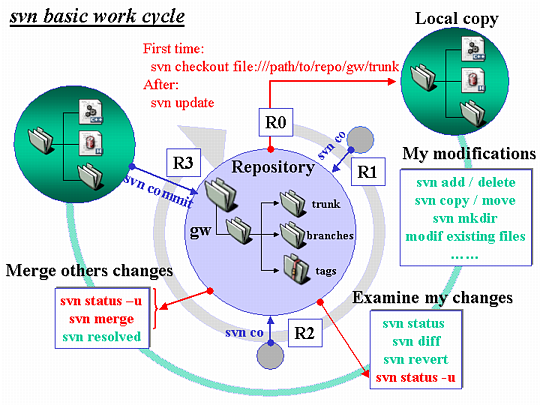
\includegraphics[height=5cm]{imgs/svnscheme.png}
\end{center}
}

\frame
{
\frametitle{Arquitectura SCV distribuido}
\begin{itemize}
 \item Todo el mundo mantiene su copia del proyecto
 \item Cada integrante del equipo trabaja en sus propias funcionalidades en su repositorio local particular
 \item El mantenedor del repositorio acepta o no las modificaciones de los integrantes
\end{itemize}

\begin{center}
 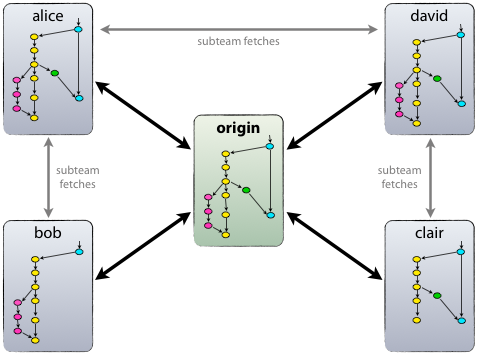
\includegraphics[height=5cm]{imgs/gitscheme.png}
\end{center}
}

\frame
{
\frametitle{GIT}
\begin{itemize}
 \item Nacido de la mente de Linus Torvalds. Versión 1.0 en 2005. 
\end{itemize}

\begin{center}
  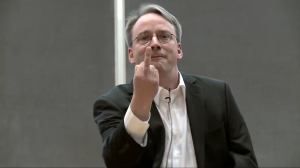
\includegraphics[height=2cm]{imgs/linus.png}    
\end{center}

\begin{itemize}
 \item Se buscaba una manera de gestionar la ingente cantidad de código del kernel de Linux
 \item Toma el diseño de versiones anteriores de BitKeeper y Monotone
 \item Git se basa en \textit{snapshots}, cada commit es una copia completa del código comprimida en binario, lo que le imprime velocidad. Usan compresión delta zlib para optimizar el espacio.
 \item Se ha medido git log frente a svn log, git opera 100x más rápido
 \item Se opera siempre en local (de ahí el incremento de velocidad) y cuando se tienen listos los cambios se suben a remoto
\end{itemize}
}


\section{Enlaces de interés}
\frame
{
\frametitle{Enlaces de interés}
\begin{itemize}
\item \url{http://nudowdeployer.wordpress.com/2013/07/23/github-vs-bitbucket-2/\#tldr}
\item \url{http://www.infoworld.com/d/application-development/bitbucket-vs-github-which-project-host-has-the-most-227061}
\item \url{http://pcottle.github.io/learnGitBranching/}
\end{itemize}
}

\end{document}